\documentclass{ctexart}
\usepackage{PhysicalChemistryNote}

\begin{document}\pagestyle{plain}
\noindent\tbf{\LARGE 6B 可逆电池的电动势}\vspace{15pt}\\
\indent 带电粒子会在电场的作用下做定向运动.对于电子而言,它总是从电势低的地方流向电势高的地方,因而形成电流.%
我们将从简单的电学和热力学出发推导电池的电动势.\\
\indent 在此之前,我们先简要介绍电势,电动势等电学中的基本概念.
\begin{definition}[6B.0.1 电势]
    电势(electric potential,简记为ePtntl)又称电位,是描述电场中某一点之能量高低性质的物理标量.%
    电场中某处的电势等于处于电场中该位置的单位电荷所具有的电势能,单位为伏特(Volt,符号为V).
\end{definition}
\begin{definition}[6B.0.2 电压]
    电压(Voltage,符号为$U$)是两点之间的电势差,也就将单位电荷从一点移动到另一点所需要的能量.
\end{definition}
\begin{definition}[6B.0.3 电动势]
    在电路学中用电动势(electromotive force,简记为emf,符号为$\mathcal{E}$或$E$)表示电源将其它形式的能量(如化学能)转化成电能的能力.%
    在电源内部,正电荷从负极被搬运至正极,电源的电动势就定义为从单位正电荷从负极移动到正极时电源提供的能量.
\end{definition}
\begin{hint}
    如果把一个闭合的电路比喻成一个循环的水流,那么电动势就是把水从低处泵到高处的水泵,%
    电动势越高就意味着水泵越有力,而电压则是水泵出水口和进水口压力差的一个表征数值.电动势表示能力属性,电压表示状态属性.
\end{hint}
电动势和电池正负极的电压由闭合电路欧姆定律关联.
\begin{theorem}[6B.0.4 闭合电路欧姆定律]
    在闭合电路中有$E=U+Ir$,其中$I$为回路电流,$r$为电池内阻,$U$为电池两极的电压.
\end{theorem}
因此,只有在回路电流$I=0$时,电池两极的电压才与电动势相等.这也是电动势测定的依据.\vspace{12pt}\\
\Section{6B.1 可逆电池}
\indent 我们在\tbf{3E.2.2}中指出,等温等压过程中系统能做的最大非体积功$W_f$等于其Gibbs自由能的减少值$\Delta G$.%
对于电池而言,这一非体积功就是电功$W_e$,Gibbs自由能的减少值就是电池反应的Gibbs自由能$\Delta_\r G$.%
由于最大功是在可逆过程中达到的,因此为了将电功与电池反应相联系,我们需要保证电池在可逆的条件下进行工作,即电池是\tbf{可逆电池}.
\begin{definition}[6B.1.1 可逆电池]
    \tbf{可逆电池}需要满足如下条件.
    \begin{enumerate}[topsep=0pt,parsep=0pt,itemsep=0pt,partopsep=0pt,label=\tbf{\arabic*.},leftmargin=*]
        \item 在无限缓慢的充放电过程中(电流趋近于零),电极反应可正向和逆向进行,电池在近平衡态的状态下工作,且能量转换可逆.
        \item 电解质中的离子迁移过程可逆.
        \item 电极反应可以逆向进行,没有不可逆的副反应(如气体析出,腐蚀等).
    \end{enumerate}
    可逆电池的电极被称作\tbf{可逆电极}.
\end{definition}
上述第一条需要外加电压才能做到,这可以与我们在\tbf{2A.3}中讨论的准静态膨胀类比.%
如果外加电压$U_\e$总是比电池电动势$\mathcal{E}$小一个无穷小量,电池就将以无穷小的电流向外放电;%
反之,如果$U_\e$总是比$\mathcal{E}$大一个无穷小量,电池就将被无穷小的电流充电.\\
\indent 如果$U_\e$与$\mathcal{E}$的差是不可忽略的常值,那么电池就将以一定的电流进行充放电.%
由于电池总是存在内阻,因此会引起发热.%
如果是向电池充电,就要向电池额外做功;如果是电池向外放电,电池向外做的功就会减少.\\
\indent 因此,以可逆的方式向电池充电消耗的电能最少,而电池以可逆的方式放电放出的电能最多.%
这和我们在讨论可逆膨胀/压缩时得出的结论是类似的,只是能量转化的形式不同.\\
\indent 我们在\tbf{6A.2}中所说的改进版的\ce{Zn-Cu}电池就可以视作可逆电池.\vspace{12pt}\\
\Section{6B.2 Nernst方程}
\Part{Nernst方程}
\indent 现在,我们来推导可逆电池的电动势.
\begin{derivation}
    假定反应体系的组成一定.根据\tbf{5B.1.1},反应的摩尔Gibbs自由能变$\Delta_\r G_\m=\pa{G}{\xi}{T,p}$.%
    于是在等温等压和该组成下,反应进行$\di\xi$时,系统的Gibbs自由能的变化为$\di G$,满足$\dfrac{\di G}{\di\xi}=\Delta_\r G_\m$.\\
    根据\tbf{3E.2.2},体系能做的最大非膨胀功(在此时即电功)为系统Gibbs自由能的变化$\di G$,于是
    \[\delta W_e=\di G=\Delta_\r G_\m\di\xi\]
    并且要求电池以可逆的方式完成此过程.\\
    假定半反应中电子的计量系数为$\nu$,那么就有物质的量为$\nu\di\xi$的电子从阳极转移到阴极.%
    由于一个电子的电荷量为$-e$,因此转移电子的总电荷量$\di Q=-\nu\e\NA\di\xi$.%
    这一过程需要对电子做的功为
    \[\delta W_e=E\di Q=-\nu Ee\NA\di\xi=-\nu FE\di\xi\]
    其中Faraday常数$F=e\NA$,即$1\mol$电子的电荷量的绝对值.\\
    结合上述两式,我们就有
    \[\Delta_\r G_\m=-\nu FE\]
    这就联系了反应Gibbs自由能变和电池的电动势.\\
    我们再考虑\tbf{5B.1.2}中标准反应Gibbs自由能变$\Delta_\r G^\ominus$和$\Delta_\r G$的关系,即
    \[\Delta_\r G_\m=\Delta_\r G^\ominus_\m+RT\ln Q\]
    代入上式可得
    \[E=-\dfrac{\Delta_\r G_\m^\ominus}{\nu F}-\dfrac{RT}{\nu F}\ln Q\]
    将有关标准反应Gibbs自由能变$\Delta_\r G_\m^\ominus$的一项定义为\tbf{标准电池电动势}$E^\ominus$,即
    \[E^\ominus=-\dfrac{\Delta_\r G_\m^\ominus}{\nu F}\]
    就有
    \[E=E^\ominus-\dfrac{RT}{\nu F}\ln Q\]
    这就是著名的Nernst方程.
\end{derivation}
\begin{theorem}[6B.2.1 Nernst方程]
    在等温等压下,某一组成时电池的电动势满足
    \[E=E^\ominus-\dfrac{RT}{\nu F}\ln Q\]
    其中\tbf{标准电池电动势}$E^\ominus$定义为
    \[E^\ominus=-\dfrac{\Delta_\r G_\m^\ominus}{\nu F}=\dfrac{RT\ln K^\ominus}{\nu F}\]
    其中$\nu$为反应转移的电子的计量数,$\Delta_\r G_\m^\ominus$为电池反应的标准摩尔反应Gibbs自由能变,$K^\ominus$为反应的标准平衡常数.
\end{theorem}
Nernst方程揭示了电池电动势与反应商$Q$之间的关联.需要注意的是,尽管反应物和产物可能被盐桥等导电物质隔离,%
反应商依然是存在的,并不要求它们混合.%
回忆我们在\tbf{5B.1.4}中的推导,是从化学势推出反应商$Q$这一概念,%
而溶质的化学势与其它溶质存在与否并无关联,只与溶质本身的浓度相关.%
这也启示我们可以把阴极和阳极分开考虑,我们将在\tbf{6C}中详细讨论这一点.\vspace{4pt}\\
\Part{热力学函数的测定}
\indent 根据Nernst方程可以将$E$与$\Delta_\r G_\m$联系起来,而电动势的测定是可以做到比较精准的%
(至少比一般的量热计要精确得多),因此测量$E$也可以间接地推定反应的热力学数据.
\begin{derivation}
    我们知道$\pa GTp=-S$,因此
    \[\pa{\Delta_\r G_\m}Tp=-\Delta_\r S_\m\]
    将Nernst方程$\Delta_\r G_\m=-\nu EF$代入可得
    \[\Delta_\r S_\m=\nu F\pa ETp\]
    又因为$\Delta_\r H_\m=\Delta_\r G_\m+T\Delta_\r S_\m$,于是
    \[\Delta_\r H_\m=-\nu FE+\nu FT\pa ETp\]
    保持压强一定,测定$E$随温度$T$的变化关系,就可以求出对应温度下的$\Delta_\r H_\m$与$\Delta_\r S_\m$.%
    需要注意的是此时测得的数据是对应于特定组成的电池的,并不是反应的标准焓变或熵变.
\end{derivation}
\Section{6B.3 电池电动势的产生原理}
\indent 一个电池总的电动势的产生是比较复杂的.我们现在来分别介绍几种主要的电动势及其产生原因.\vspace{4pt}\\
\Part{电极与电解质溶液界面电势}
\indent 金属晶格中有金属离子和能够自由移动的电子存在\footnote{你应当在结构化学中学习过这一点.}.%
当我们把金属单质\ce{M}浸入含对应金属离子\ce{M^n+}的溶液时,如果\ce{M^n+}在金属中和在溶液中的化学势不相等,%
就会发生转移.根据溶液中\ce{M^n+}浓度的不同,这可能发生两种情形:\ce{M^n+}从单质转移至溶液,电子留在单质中;%
使得金属带负电,溶液带正电;%
或是\ce{M^n+}从溶液转移至单质,使得溶液带负电,金属带正电.\\
\indent 无论何种情形,都会导致两相带上相反的电荷,从而使得界面出现电势差.%
同时,由于静电作用,这一电势差会阻止金属离子继续发生转移,从而很快地达成平衡,于是两相的电势差也趋于稳定.\\
\indent 在静电作用下,金属相所带的电荷是集中在表面的,而溶液中的带异号电荷的离子一方面受到金属表面电荷的吸引,趋向于紧靠金属表面;%
另一方面,离子的热运动使得它们又会趋向于平均地分布在溶液中.%
当静电吸引与热运动分散平衡时,在电极与溶液界面处就形成了一个\tbf{双电层}\footnote{双电层最早由Helmholtz提出并模型化,在不断优化下形成Gouy-Chapman-Stern模型.%
关于双电层理论的演化历史,可以参考https://zhuanlan.zhihu.com/p/27155545.}.
\begin{definition}[6B.3.1 双电层]
    \tbf{双电层}是由电极表面上的电荷层与溶液中过剩的反号离子层构成,这一离子层又分为\tbf{紧密层}和\tbf{扩散层}两部分.%
    与金属靠的较为紧密的一层称为紧密层,除此之外扩散到溶液中去的称为扩散层.
\end{definition}
一般而言,紧密层的厚度约为$0.1\text{ nm}$,而扩散层的厚度与溶液的浓度,金属的电荷以及温度等有关.%
溶液浓度越大,分散层厚度越小,其厚度通常在$10^{-10}\sim10^{-6}\text{m}$之间.\\
\indent 如果规定溶液本体中的电位为$0$,电极相的电位为$\ep$,则电极与溶液界面电势差就是$\ep$.$\ep$在双电层中的分布情况如下图所示,%
是紧密层电位$\psi_1$和扩散层电位$\psi_2$的加和值.
\begin{tightcenter}
    \documentclass{standalone}
\usepackage{PhysicalChemistryNote}
\begin{document}
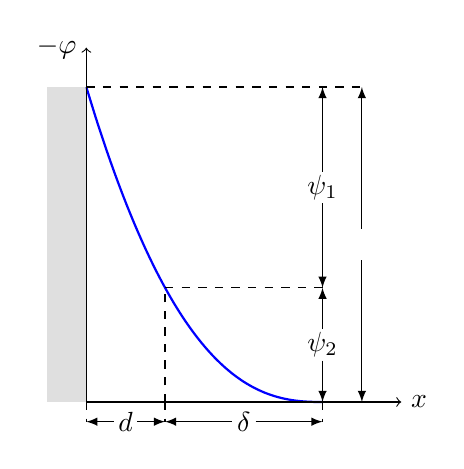
\begin{tikzpicture}
    \draw[domain=0:3,thick,blue] plot[smooth](\x,{(3-\x)^(2.5)/(3^2.5)*4});
    \draw[->] (0,0)--(4,0) node[right]{$x$};
    \draw[->] (0,0)--(0,4.5) node[left]{$-\varphi$};
    \draw[dashed] (1,0)--(1,{(2^2.5)/(3^2.5)*4});
    \draw[dashed] (0,4)--(3.5,4);
    \draw[dashed] (1,{(2^2.5)/(3^2.5)*4})--(3,{(2^2.5)/(3^2.5)*4});
    \draw[dashed] (1,0)--(1,-0.25);
    \draw[dashed] (3,0)--(3,-0.25);
    \draw[dashed] (0,0)--(0,-0.25);
    \node at (3,{(2^2.5)/(3^2.5)*2}) {$\psi_2$};
    \node at (3,{(2^2.5)/(3^2.5)*2+2}) {$\psi_1$};
    \node at (3.5,2) {$\ep$};
    \node at (0.5,-0.25) {$d$};
    \node at (2,-0.25) {$\delta$};
    \draw[-latex] (3,{(2^2.5)/(3^2.5)*2-0.2})--(3,0);
    \draw[-latex] (3,{(2^2.5)/(3^2.5)*2+0.2})--(3,{(2^2.5)/(3^2.5)*4});
    \draw[-latex] (3,{(2^2.5)/(3^2.5)*2+1.8})--(3,{(2^2.5)/(3^2.5)*4});
    \draw[-latex] (3,{(2^2.5)/(3^2.5)*2+2.2})--(3,4);
    \draw[-latex] (3.5,1.8)--(3.5,0);
    \draw[-latex] (3.5,2.2)--(3.5,4);
    \draw[-latex] (2.15,-0.25)--(3,-0.25);
    \draw[-latex] (1.85,-0.25)--(1,-0.25);
    \draw[-latex] (0.65,-0.25)--(1,-0.25);
    \draw[-latex] (0.35,-0.25)--(0,-0.25);
    \fill[lightgray,opacity=0.5] (-0.5,0)rectangle(0,4);
\end{tikzpicture}
\end{document}
\end{tightcenter}
图中的灰色区域表示金属,横坐标$x$为距离金属表面的距离,纵坐标$-\phi$为对应位置的负电势.\\
\indent 事实上,我们将在\tbf{6B.3}中讨论的电极电势指的就是电极与电解质溶液的界面电势.%
关于这一点,之后会给出更详细的解释.\vspace{4pt}\\
\Part{接触电势}
\indent 对于不同的金属,其电子具有的能量也不同,Fermi能级\footnote{音译为费米.$0\K$下Fermi能级定义为电子能占据的最高能级,在一般温度下Fermi能级定义为电子有50\%概率占据的能级.%
简单来说,Fermi能级衡量了一个系统中电子的平均能量,当两个系统接触时电子将从Fermi能级高的系统移动至Fermi能级低的系统,直至两个系统的Fermi能级相同.这一概念与系统的化学势有十分密切的关联.\\
\indent 关于Fermi能级的形象概念,你也可以参考https://www.zhihu.com/question/22560362/answer/2180449510.}也不同.%
当这两种不同的金属接触时,电子会从Fermi能级高的金属流入Fermi能级低的金属,直至达到平衡.%
这一过程会使得两种金属带上相反的电荷,从而使得界面出现电势差.这就是\tbf{接触电势}.
\begin{definition}[6B.3.2 接触电势]
    \tbf{接触电势}是由于两个或多个材料接触面上存在不同程度的电子互相转移和表面电荷分布不均所产生的电势差.
\end{definition}
由于我们一般要用导线将两个电极相连,而导线又以铜质导线居多,因此接触电势在大部分情况下都是存在的.\vspace{4pt}\\
\Part{液体接界电势}
\indent 液体接界电势,即我们在\tbf{6A.2}所说的\tbf{液接电势},是由于两个组成不同的溶液之间存在离子扩散速率的差异导致的.%
例如在两种浓度不同的\ce{HCl}溶液的界面上,由于\ce{H^+}的扩散速率明显快于\ce{Cl^-},%
因此越过界面的\ce{H^+}就比\ce{Cl^-}多,使较稀的一侧出现过量\ce{H^+},%
较浓的一侧剩余过量\ce{Cl^-},从而使得界面出现电势差.%
这一电势差反过来会加速\ce{Cl^-}的扩散,减缓\ce{H^+}的扩散,%
最终两种离子扩散速率相等时的电势差即为\tbf{液接电势}.
\begin{definition}[6B.3.2 液体接界电势]
    \tbf{液体接界电势}是由于组成不同的溶液界面上各种离子扩散速率不同所产生的电势差.
\end{definition}
为了减小液体接界电势的影响,我们通常在两个溶液之间用盐桥连接,使液接电位降低或接近于消除.%
以饱和\ce{KCl}盐桥为例,由于其浓度很高,因此盐桥与两边溶液各自的界面上主要发生\ce{K^+}和\ce{Cl^-}的扩散.%
由于\ce{K^+}和\ce{Cl^-}的扩散速率几乎相等,所以在两个界面上只会产生两个数值很小且几乎相等,方向相反的液接电位,%
从而在很大程度上减小液接电势.\vspace{4pt}\\
\Part{电池电动势的组成}
\indent 上述几种电势共同组成了电池的电动势.以\ce{Zn-Cu}电池为例,其电池电动势的来源为
\vspace{-5pt}\begin{table}[H]\centering
    \begin{tabular}{ccccccccc}
        \ce{Cu(s)} &$\vert$ &\ce{Zn(s)}   &$\vert$ &\ce{ZnSO4(aq)} &$\vert$    &\ce{CuSO4(aq)} &$\vert$    &\ce{Cu(s)}\\
                &$\varphi_{\text{接触}}$    &&$\ep_{-}$&&$\varphi_{\text{液接}}$&&$\ep_{+}$
    \end{tabular}
\end{table}\vspace{-15pt}
为了表示接触电势,将与\ce{Zn}相连的\ce{Cu}写在最左边.这样,电池的电动势$E$就满足
\[E=\varphi_{\text{接触}}+\varphi_{\text{液接}}+\ep_-+\ep_+\]
虽然$\ep_-$和$\ep_+$的值难以测量,但我们在\tbf{6C}中将介绍电极电势,以此将$\ep$转化为一个可测的常量.\vspace{12pt}\\
\Section{6B.4 电动势的测定\footnote{本节内容仅需了解即可,不必掌握.}}
\Part{Poggendorff对消法测电动势}
\indent 可逆电池的电动势不能直接用电压表来测定.使用电压表读数时,回路中有一定的电流,%
这使得此时的电池并不是可逆电池,并且测得的也只是电池的正负极电压而非其电动势.%
因此,测定可逆电池的电动势需要在几乎没有电流通过的情况下进行.
\begin{center}
    \documentclass{standalone}
\usepackage{PhysicalChemistryNote}
\begin{document}
\begin{tikzpicture}
    \draw[-] (0,0)--(1,0);
    \draw[-] (1.9,-1)--(1,-1)--(1,1)--(1.9,1);
    \draw[-] (2.1,-1)--(3,-1)--(3,-0.25);
    \draw[-] (3,0.25)--(3,1)--(2.1,1);
    \draw[-] (3,0.25)--(3.5,0)--(4.7,0);
    \draw[-] (5.3,0)--(6.5,0);
    \draw[-latex] (6.5,0)--(6.5,2.85);
    \draw[-] (0,0)--(0,3)--(2,3);
    \draw[-] (9,3)--(10,3)--(10,4);
    \draw[-] (0,3)--(0,4)--(2.9,4);
    \draw[-] (3.1,4)--(6.5,4);
    \draw[-] (7.5,4)--(10,4);
    
    \draw[thick] (5,0) circle (0.3);
    \draw[draw=black,fill=white] (3.5,0) circle (0.05);
    \draw[draw=black,fill=white] (3,-0.25) circle (0.05);
    \draw[draw=black,fill=white] (3,0.25) circle (0.05);
    \draw[draw=black,fill=white,thick] (2,2.85)rectangle(9,3.15);
    \draw[draw=black,fill=white,thick] (6.5,3.85)rectangle(7.5,4.15);
    \draw[-latex] (6.6,3.6)--(7.4,4.4);

    \draw[-,thick] (1.9,0.85)--(1.9,1.15);
    \draw[-,thick] (2.1,0.75)--(2.1,1.25);
    \draw[-,thick] (1.9,-0.85)--(1.9,-1.15);
    \draw[-,thick] (2.1,-0.75)--(2.1,-1.25);
    \draw[-,thick] (2.9,3.85)--(2.9,4.15);
    \draw[-,thick] (3.1,3.75)--(3.1,4.25);

    \node at (2,1.5) {$E_x$};
    \node at (2,-1.5) {$E_{\text{s.c.}}$};
    \node at (3,4.5) {$E_{w}$};
    \node at (7,4.5) {$R$};
    \node[below right] at (3.5,0) {$K$};
    \node at (5,0) {$G$};
    \node[below] at (2,2.85) {$A$};
    \node[below] at (9,2.85) {$B$};

\end{tikzpicture}
\end{document}
\end{center}
Poggendorff对消法就是依据上述条件设计的测定电源电动势的方法,其电路图如上所示.%
我们现在来介绍其具体步骤.
\begin{solution}
    工作电源$E_w$在均匀的电阻丝$AB$上产生均匀的压降(这可以由欧姆定律得出).\\
    首先将开关$K$打到上端,使得待测电源$E_x$接入电路.调节$AB$上的滑动点,使得灵敏电流计$G$的示数为$0$.%
    记此时滑动点的位置为$X$,则由于电流$I=0$而$E_x$的电动势与$AX$上的电压相等.\\
    现在将开关$K$打到下端,使得标准电源$E_{\text{s.c.}}$接入电路.同样调节滑动电使$G$的实数为$0$,%
    记此时滑动点的位置为$P$.这样,$E_{\text{s.c.}}$的电动势与$AP$上的电压相等.\\
    考虑上半部分电路的欧姆定律,有
    \[E_x=U_{AX}=I_wR_{AX}=I_w\rho\dfrac{\overline{AX}}{S}\]
    \[E_{\text{s.c.}}=U_{AP}=I_wR_{AP}=I_w\rho\dfrac{\overline{AP}}{S}\]
    其中$\rho$为电阻丝的电阻率,$S$为其横截面积.这样就有
    \[E_x=\dfrac{\overline{AX}}{\overline{AP}}E_{\text{s.c.}}\]
    测定相关的长度,就可以由标准电池的电动势得到待测电池的电动势.
\end{solution}
\Part{Weston标准电池}
\indent 我们在Poggendorff对消法中需要一个电势已知的标准电池.常用的标准电池是\tbf{Weston标准电池},%
可以表示如下.
\[\ce{Cd(Hg)}\vert\ce{CdSO4.8/3H2O(s)}\vert\ce{CdSO4(aq)}\vert\ce{CdSO4.8/3H2O(s)}\vert\ce{Hg,Hg2SO4}\vert\ce{Hg}\]
电池的负极为镉汞齐,正极是\ce{Hg}与\ce{Hg2SO4}的混合糊状物.为了正极与导线更好接触,在正极下再置入一层\ce{Hg}单质.%
正极和负极表面均覆盖有$\displaystyle\ce{CdSO4.8/3H2O(s)}$,然后用\ce{CdSO4}饱和溶液连接两极.\\
\indent 电池的电动势是稳定的,并且只与镉汞齐中\ce{Cd}的活度有关,%
而\ce{Cd}的活度在一定温度下是定值.因此,Weston标准电池的电动势只与温度$T$有关.%
根据温度查阅相关数据即可得出其电动势.
\end{document}